\documentclass{beamer}
\usepackage[latin1]{inputenc}
\usepackage{fixltx2e}
\usepackage{hyperref}
\usepackage{graphicx}

\graphicspath{ {img/} }

\usetheme{Hannover}


\title[Large data in python]{What to do when your data are \textbf{large} \\ but not \texttt{big}}
\author{Dillon Niederhut}
\institute{PyBay -- the San Francisco Bay Area Python Conference}
\date{20 August 2016}
\begin{document}

\begin{frame}
\titlepage
\end{frame}

\AtBeginSubsection[]
{
  \begin{frame}<beamer>
    \frametitle{Layout}
    \tableofcontents[currentsection,currentsubsection]
  \end{frame}
}


\section{Introduction}

\begin{frame}{about this talk}
    \begin{itemize}
        \item data at \href{https://github.com/deniederhut/pybay_2016}{github.com/deniederhut/pybay\_2016}
        \item python libraries : \texttt{celery, h5py, numpy, pandas, pymongo}
        \item other libraries : \texttt{mongodb, rabbitmq, sqlite}
    \end{itemize}
\end{frame}

\begin{frame}{about me}
    \begin{figure}
        \centering
        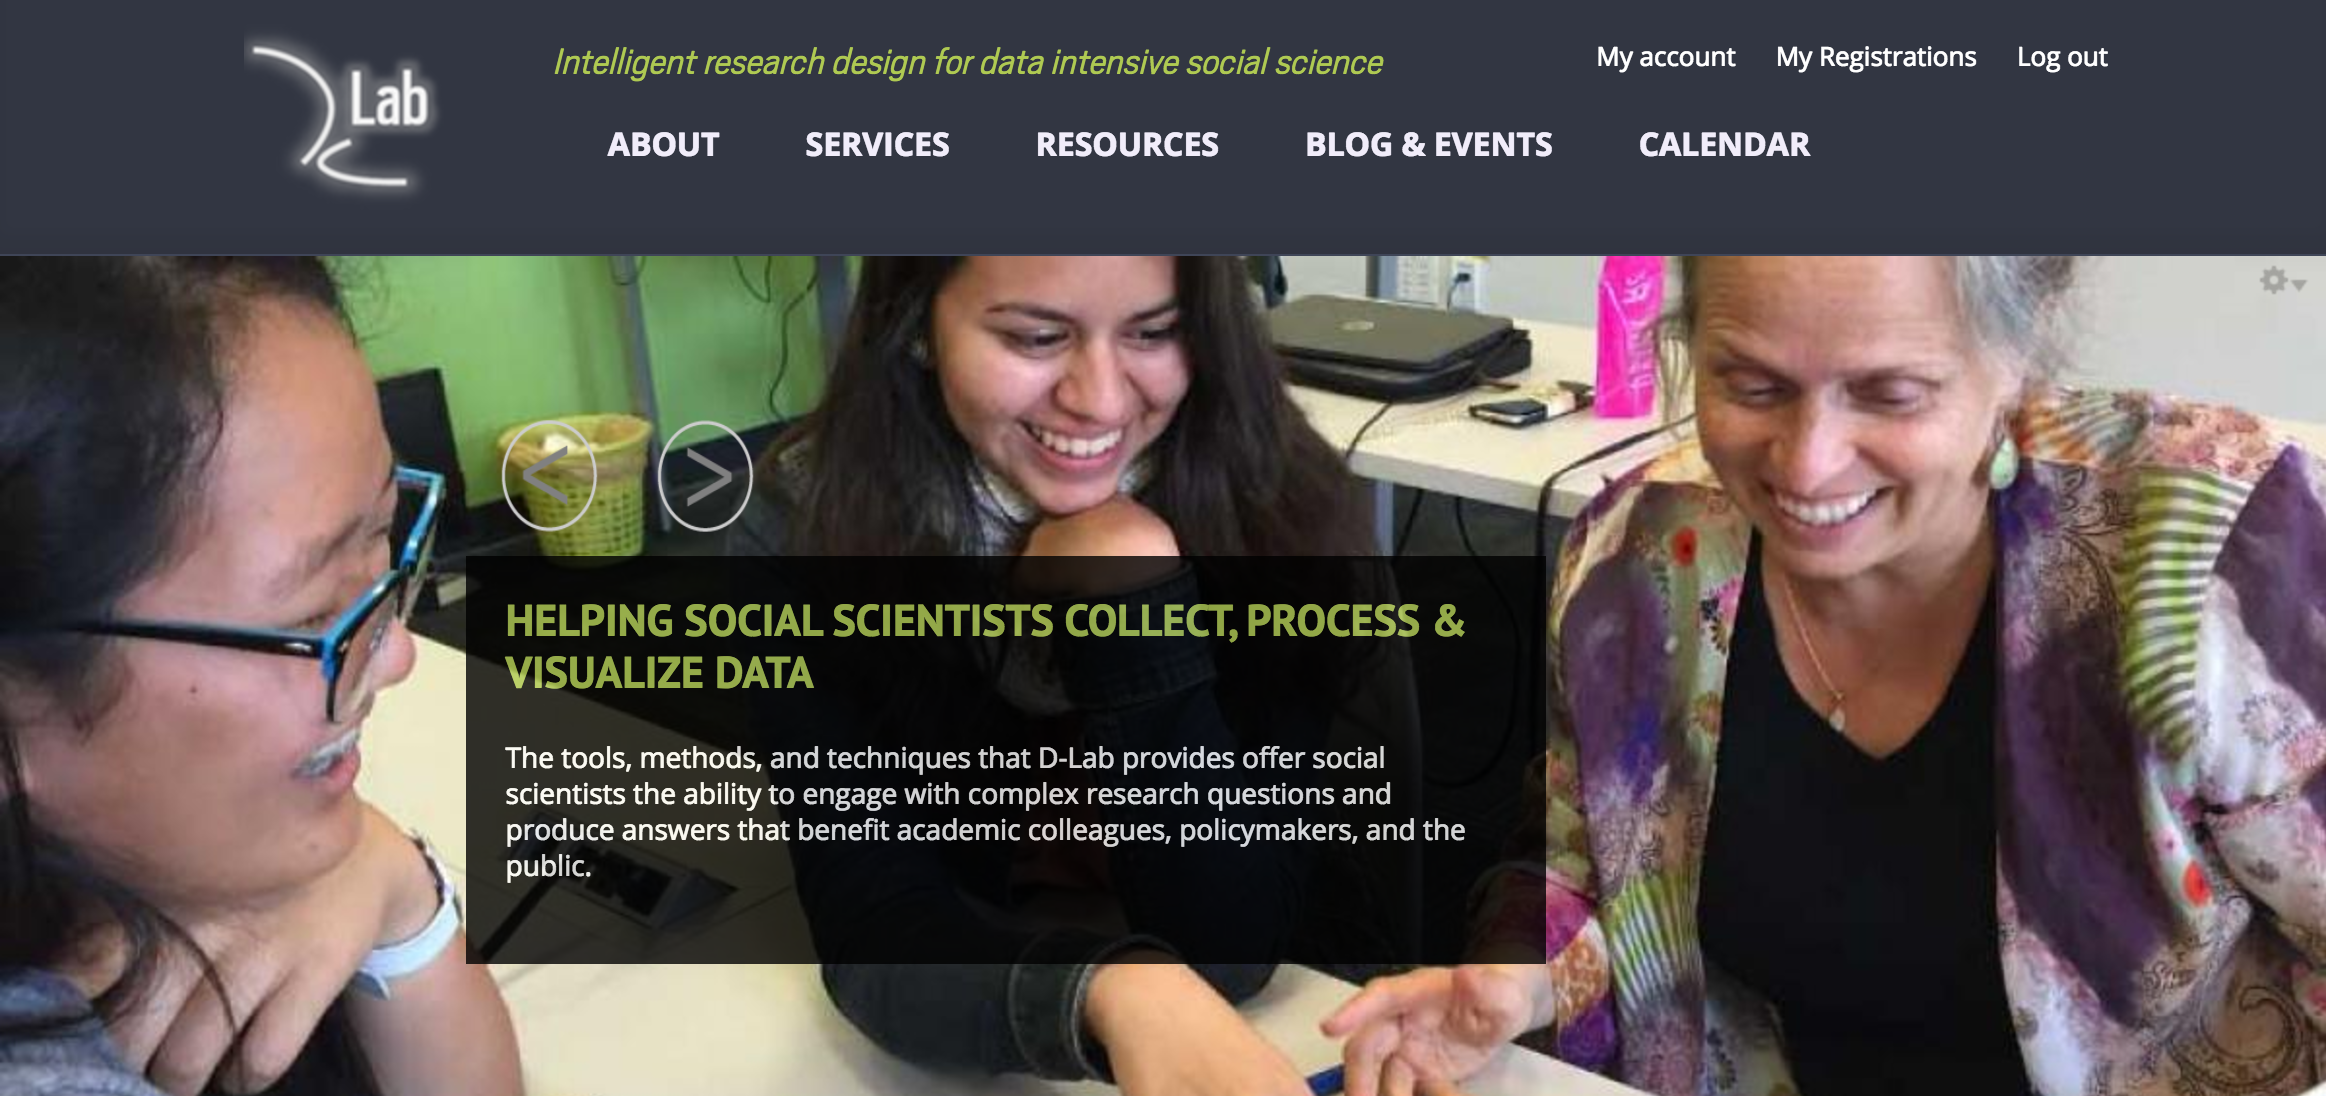
\includegraphics[width=\textwidth]{dlab.png}
    \end{figure}
    \begin{itemize}
        \item \href{https://dlab.berkeley.edu}{dlab.berkeley.edu}
        \item \href{https://twitter.com/DLabAtBerkeley}{@DLabAtBerkeley}
    \end{itemize}
\end{frame}


\section{Motivation}

\begin{frame}{size concerns}
    \begin{figure}
        \centering
        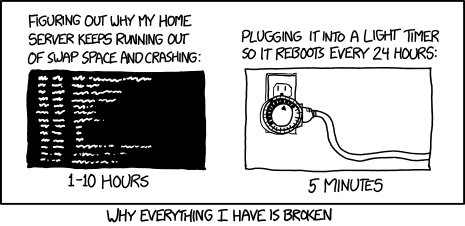
\includegraphics[width=\textwidth]{hard_reboot.png}
        \footnote{\href{http://xkcd.com}{from xkcd}}
    \end{figure}
\end{frame}

\begin{frame}{time concerns}
    \begin{figure}
        \centering
        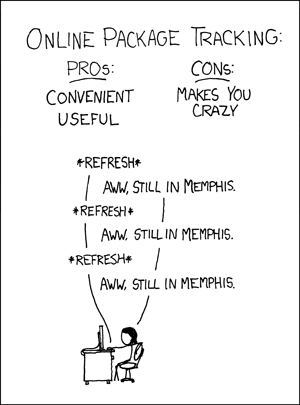
\includegraphics[width=5cm]{online_package_tracking.png}
        \footnote{\href{http://xkcd.com}{always relevant}}
    \end{figure}
\end{frame}

\begin{frame}{code concerns}
    \begin{figure}
        \centering
        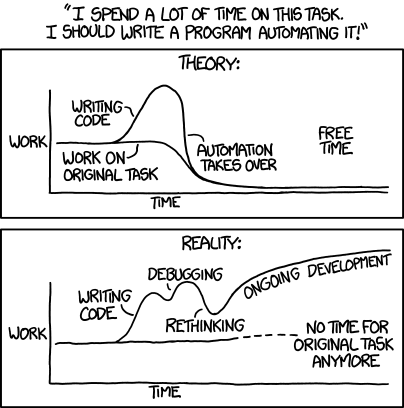
\includegraphics[width=6.5cm]{automation.png}
        \footnote{\href{http://xkcd.com}{thanks Randall!}}
    \end{figure}
\end{frame}


\section{Strategies}

\begin{frame}{sequential processing}
    \begin{figure}
        \centering
        
\includegraphics[width=\textwidth]{chunk.png}
    \end{figure}
\end{frame}

\begin{frame}{parallel processing}
    \begin{figure}
        \centering
        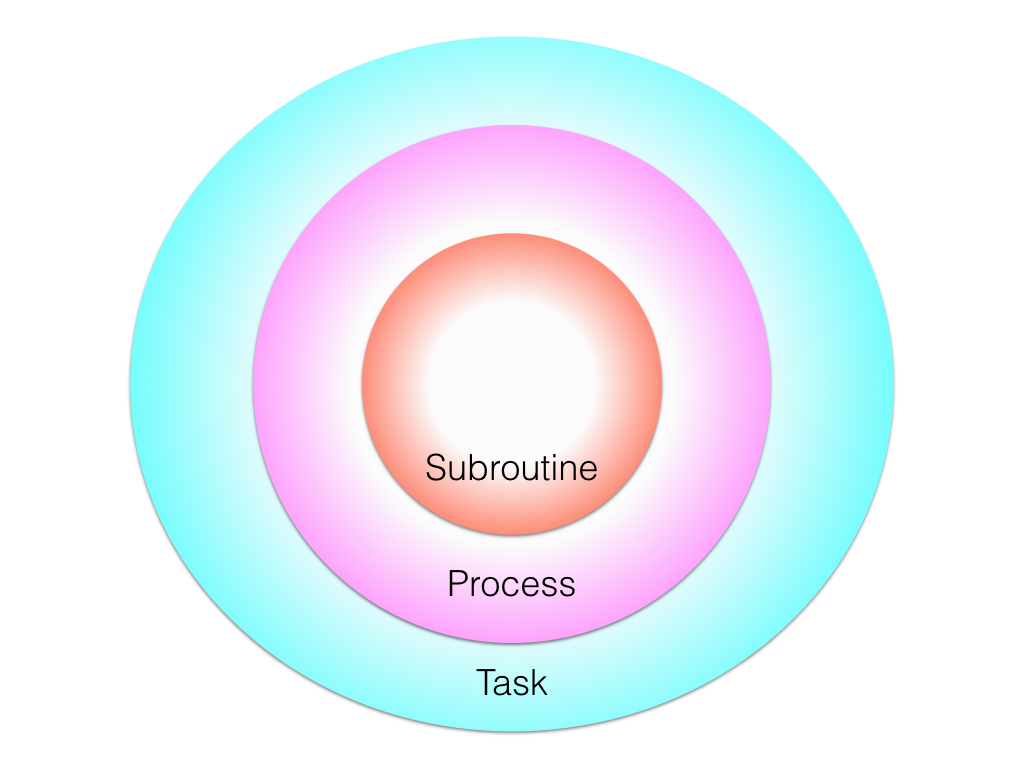
\includegraphics[width=\textwidth]{parallel.png}
    \end{figure}
\end{frame}


\section{Closing}

\begin{frame}{contact}
    \begin{figure}
        \centering
        
\includegraphics[width=\textwidth]{enthought.png}
    \end{figure}
\begin{itemize}
    \item \href{http://dillon.niederhut.us}{dillon.niederhut.us}
    \item \href{https://twitter.com/dillonniederhut}{@dillonniederhut}
\end{itemize}
\end{frame}

\end{document}
